\documentclass[a4paper]{leaflet}

\usepackage[T1]{fontenc}
\usepackage[utf8]{inputenc}
\usepackage[french]{babel}
\usepackage{rotating}

\newcommand{\ei}{\textperiodcentered}
\begin{document}
\begin{titlepage}
  \title{
    Soutenance de thèse d'Arnald Sengers
    \date{19/07/2019} \\
    \textsc{Schémas semi-implicites et de diffusion-redistanciation pour la dynamique des globules rouges.}\\[1cm]    
    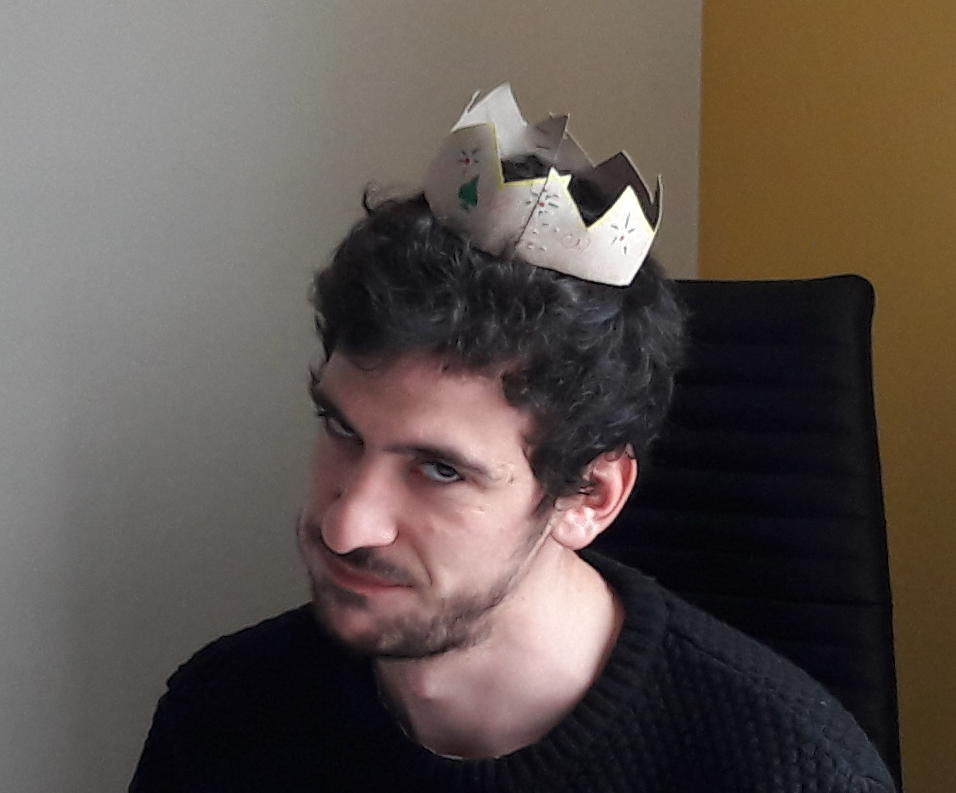
\includegraphics[width=0.5\textwidth]{crop}
} % sous la direction de: \\
% Emmanuel MAÎTRE
% Mourad ISMAIL
% Thibaut JECONNAISPASLENOM

\end{titlepage}

\maketitle

\newpage
\section*{Résumé}
Dans ce travail, nous nous sommes intéressés à la mise en place de schémas semi- implicites pour l'amélioration des simulations numériques du déplacement d'un globule rouge dans le sang. Nous considérons la méthode levelset où l'interface fluide-structure est représentée comme la ligne de niveau 0 d'une fonction auxiliaire et le couplage est effectué en ajoutant un terme source dans l'équation fluide. Le principe de ces schémas semi-implicites est de prédire la position et la forme de la structure par une équation de la chaleur et d'utiliser cette prédiction pour obtenir un terme de force plus précis dans l'équation fluide. Ce type de schémas semi-implicites a d'abord été mis en place dans le cadre d'un système diphasique ou d'une membrane élastique immergée pour avoir des conditions moins restrictives sur le pas de temps que pour un couplage explicite. Cela a permis d'en choisir un plus grand et ainsi augmenter l'efficacité globale de l'algorithme complet par rapport à un schéma explicite classique. Afin d'étendre ce raisonnement au cas d'un globule rouge, nous proposons un algorithme pour simuler le flot de Willmore en dimensions 2 et 3. Notre méthode s'inspire des méthodes de mouvements d'interface générés par diffusion et nous arrivons à obtenir un flot non linéaire d'ordre 4 uniquement avec des résolutions d'équations de la chaleur. Pour assurer la conservation du volume et de l'aire d'un globule rouge, nous proposons ensuite une méthode de correction qui déplace légèrement l'interface afin de recoller aux contraintes. La combinaison des deux étapes précédentes décrit le comportement d'un globule rouge laissé au repos. Nous validons cette méthode en obtenant une forme d'équilibre d'un globule rouge. Nous proposons enfin un schéma semi-implicite dans le cas d'un globule rouge qui ouvre la voie vers l'utilisation de cette méthode comme prédicteur de l'algorithme de couplage complet.
\section*{Résumé vulgarisé}
Faire des simulations de globules rouge pose pleins de problèmes: un globule est élastique et donc sa forme a tendance à changer avec le temps et le fluide dans lequel il se trouve. Cela impose d'être très précautionneux quand on fait tourner ces simulations sur ordinateur, et donc cela prend très longtemps sur des machines puissantes. Heureusement, Arnaud a pu travailler dessus, ce qui permet d'être plus efficace.

\section*{Déroulement de la soutenance}
La soutenance se déroule en plusieurs étapes:
\begin{itemize}
\item la soutenance en elle-même ($\approx$ 40min)
  le\ei la candidat\ei e présente de manière concise ses travaux.
  \textbf{NE PAS APPLAUDIR À LA FIN DE LA PRÉSENTATION}
  il est possible de partir à ce moment, car souvent les questions sont très pointues et la durée peut être variable
\item les questions du jury ($\approx$ 30 min, 1h):
  Le jury interroge le\ei la candidat\ei e sur ses travaux, sur la présentation et le manuscrit de thèse qu'il\ei elle leur aura envoyé auparavant.
\item la délibération ($\approx$ 1h):
  Le\ei la candidat\ei e peut souffler, pendant que le jury se réunit dans une pièce à part, afin de décider de l'obtention ou non du titre de docteur\ei e, mais aussi de l'appréciation inscrite sur le procès-verbal.
\item l'annonce du résultat et les remerciements:
  Le jury sort de la pièce, et énonce le contenu du PV. Le\ei la candidat\ei e peut maintenant faire ses remerciements
\item le pot de thèse
  le\ei la candidat\ei e part remercier personnellement les membres du jury, tandis qu'il est enfin possible de profiter du traditionnel buffet et des boissons. C'est aussi à ce moment là qu'il est possible de remarquer les gens qui n'ont pas assisté à la soutenance
\end{itemize}

\section*{Passé glorieux: Standing on the shoulders of giants}

Et si nous nous intéressions un petit peu aux descendants d'Arnaud...

Nous savons tous qu'Emmanuel Maitre est le père mathématique et spirituel d'Arnaud. Merci à lui d'ailleurs de l'avoir nourri d'équations, abreuvé de C++, pour le faire grandir en ce beau futur docteur qu'est devenu Arnaud ! 

Mais saviez-vous qu'en remontant ainsi son arbre généalogique mathématique, de très grand noms figurent parmi sa famille. Je ne vous en citerai que quelques-uns, tels Hermite, Chasles, Poisson, Euler, ou même\dots Copernic lui-même ! Si si, croix de bois, croix de fer. On se permettra également de parler de ce cher Léonard (de Vinci), que j'ai entendu Arnaud appeller une fois son \og cher grand-tonton\fg. Bon, on vous a assez hypé comme ça, n'hésitez pas à vous référez à l'arbre généalogique simplifié de notre doctorant préféré pour en apprendre plus sur lui. 

\begin{figure}
	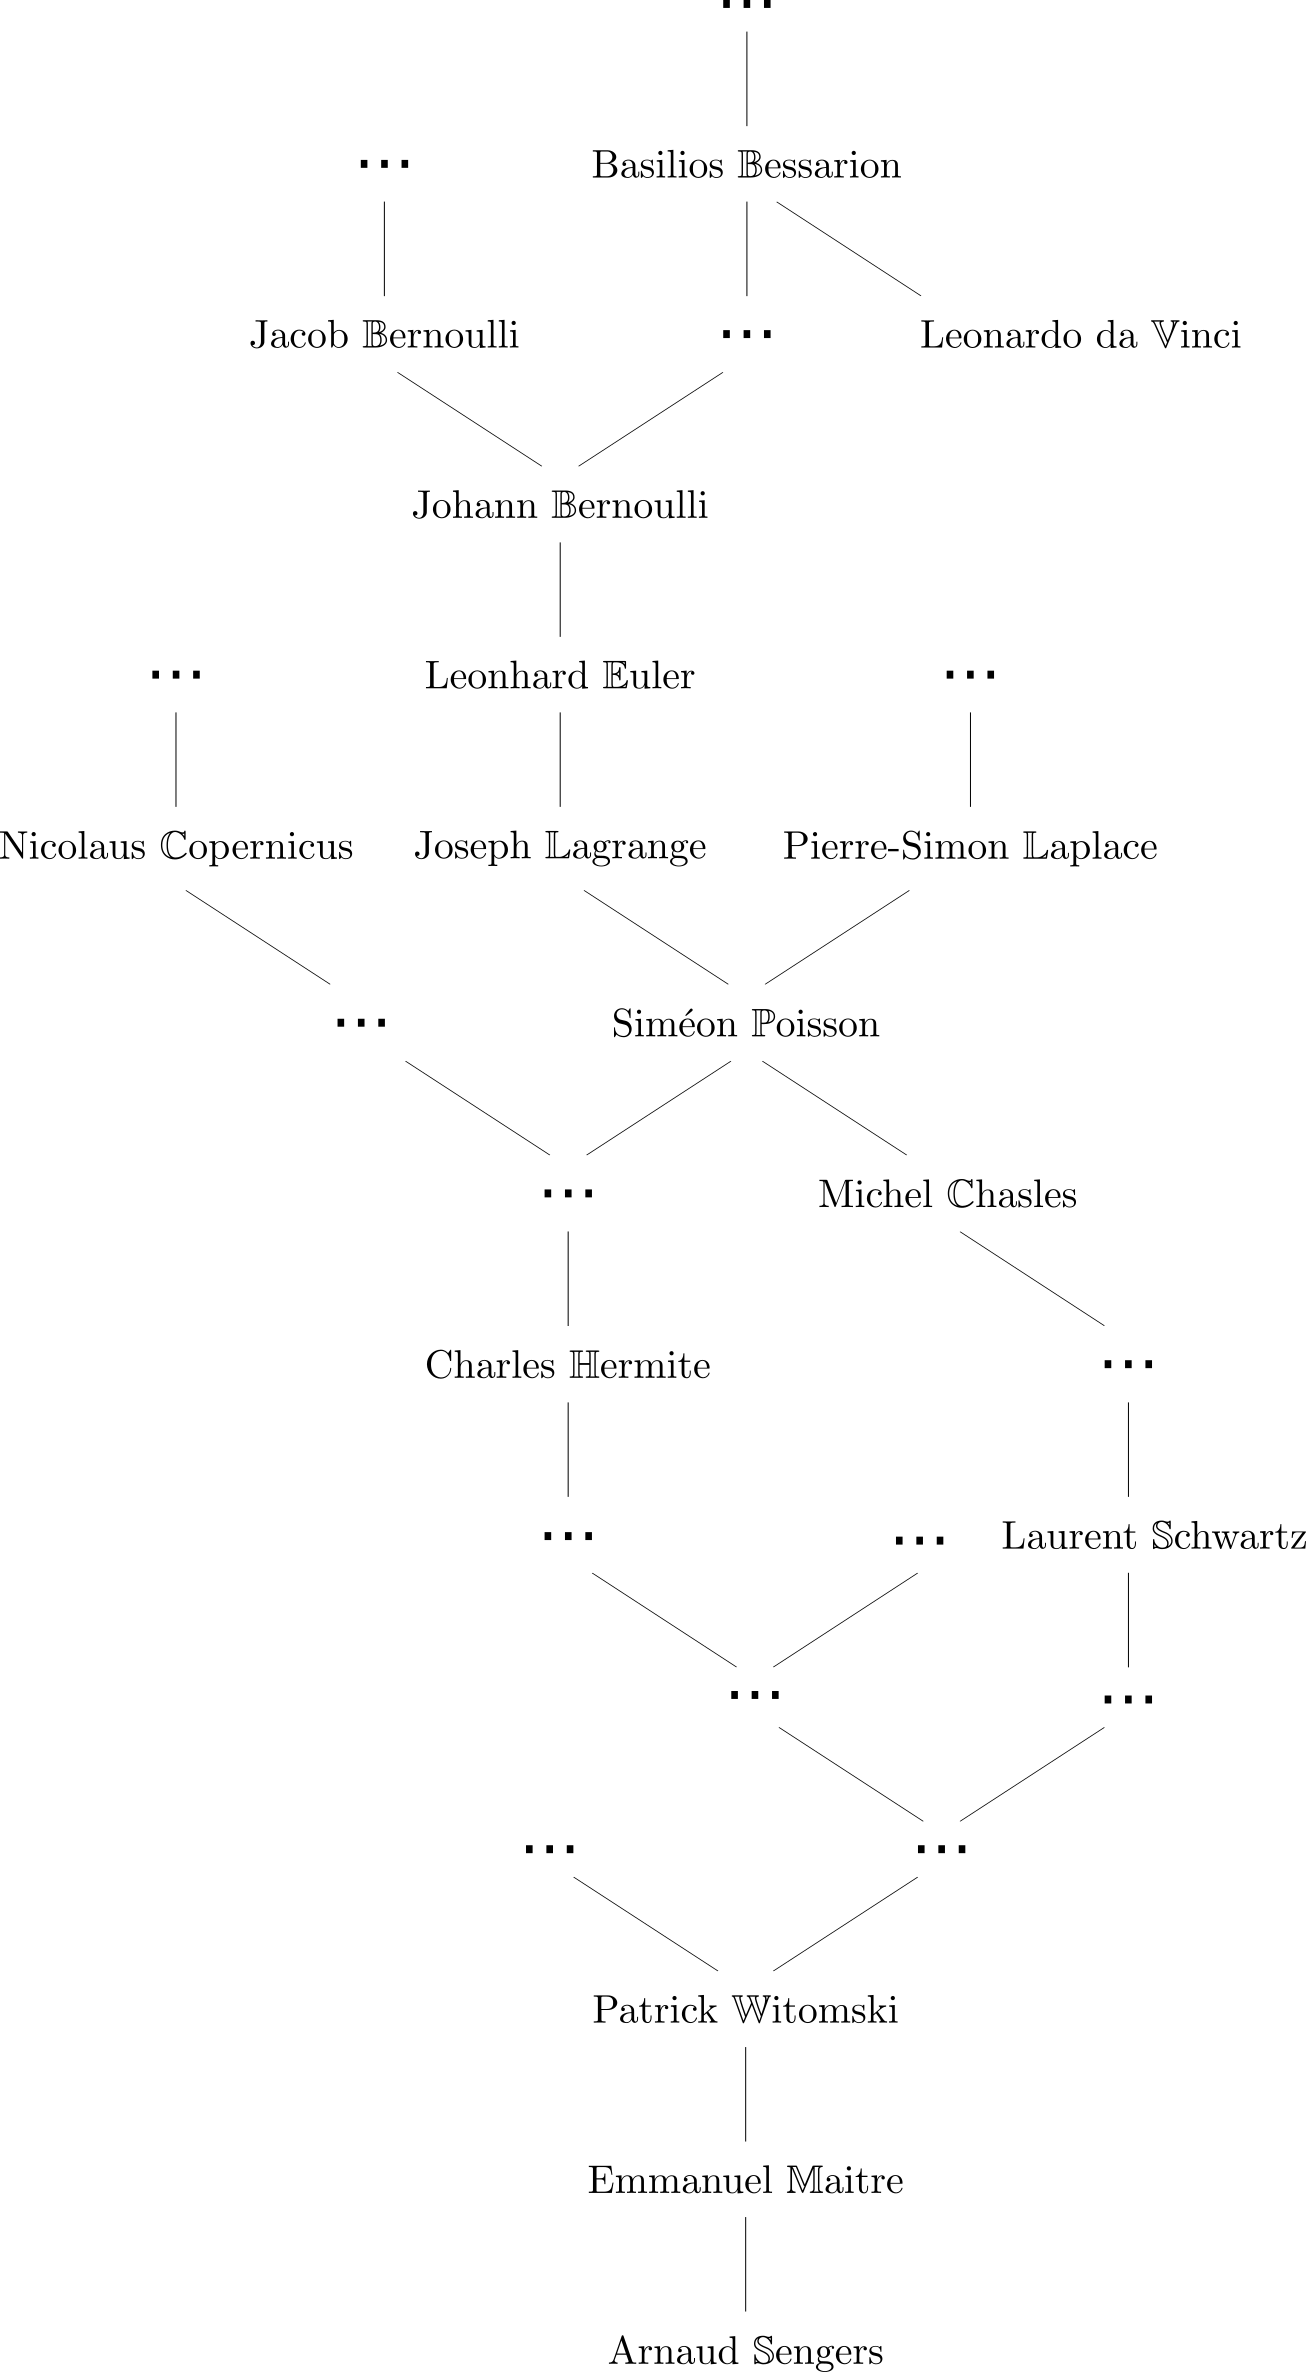
\includegraphics[width=\textwidth]{genealogie.png}
	\caption{Découvre tous les fameux ancêtres d'Arnaud}
\end{figure}


\section*{Le saviez-vous}
\begin{itemize}
\item Le séminaire des doctorants donné par Arnaud le mercredi 27/06/2018 a été celui qui a enregistré la plus grande affluence en 2 ans
\item L'équipe de foot du LJK coachée par Arnaud a atteint les 8èmes de finales du tournoi inter-labos
\item Arnaud s'est un jour fait battre à la course à pied par un ancien doctorant, mais cela n'a jamais été vérifié % peut etre trop private joke
\item Arnaud possède une connaissance sommaire du latin et du grec ancien
\end{itemize}


\section*{Loisirs}
Le temps peut parfois paraître un peu long durant cette demi-journée:

\begin{itemize}
\item Compter le nombre de fois que Arnaud dit ``Essentiellement'': $\dots$
\end{itemize}

\begin{table}[!h] % Idées bingo ?
  \centering
  \begin{tabular}{*3{|c}|}\hline
    ``Flot de Willmore''& Quinte de toux & Pause boisson  \\ \hline
    Qqun s'endort & & Qqchose tombe\\ \hline
  \end{tabular}
  \caption{Bingo}
\end{table}

\begin{figure}
	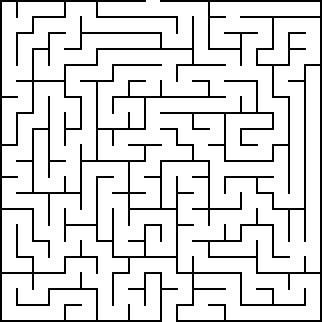
\includegraphics[width=\textwidth]{maz.png}
	\caption{Aidez Arnaud à avoir sa thèse}
\end{figure}

\end{document}



%%% Local Variables:
%%% mode: latex
%%% TeX-master: t
%%% End:
